% voodoo for arXiv scripts
\pdfoutput=1
\documentclass[aps,prd,twocolumn,superscriptaddress,preprintnumbers,floatfix,nofootinbib]{revtex4-2}

\usepackage{graphicx}
\usepackage{amsmath}
%\usepackage{mdwlist}
%\usepackage[caption=false]{subfig}
%\usepackage{siunitx}
%\usepackage{placeins}
\usepackage{color}
%\usepackage{standalone}
\usepackage{dcolumn}
\usepackage{tensor}
\usepackage{bm}
\usepackage{makecell}
%\usepackage{MnSymbol}
\usepackage[T1]{fontenc}
\usepackage[utf8]{inputenc}
\usepackage{microtype}
\usepackage{etoolbox}
\usepackage{amssymb}
\usepackage{mathrsfs}
\usepackage{accents}
\usepackage[normalem]{ulem}
\usepackage[table,dvipsnames]{xcolor}
\usepackage[colorlinks,urlcolor=NavyBlue,citecolor=NavyBlue,linkcolor=NavyBlue,pdfusetitle]{hyperref}
\usepackage[all]{hypcap}
\usepackage[inline,shortlabels]{enumitem}
\usepackage{braket}

\usepackage{array}
\usepackage{diagbox}
\usepackage{color}
\usepackage{colortbl}
\usepackage{hhline}
\usepackage{multirow}

\graphicspath{{./}{figs/}}

\newcommand{\nn}{\nonumber}
\newcommand{\NR}{\text{NR}}

\def\N{{\cal N}}
\def\M{{\cal M}}

\newcommand{\lorena}[1]{\textcolor{RoyalPurple}{#1}}
\newcommand{\simone}[1]{\textcolor{JungleGreen}{#1}}
\newcommand{\sa}[1]{{\textcolor{green}{\texttt{SA: #1}} }}  % command used for comments 

%%%%%%%%%%%%%%%%%%%%%%%%%%%%%%%%%%%%%%%%%%%%%%%%%%%%%%%%%%%%
%% Author information
%!TEX encoding = UTF-8 Unicode
%%%%%%%%%%%%%%%%%%%%%%%%%%%%%%%%%%%%%%%%%%%%%%%%%%%%%%%%%%%%


\usepackage{orcidlink}

\newcommand{\MST}{\affiliation{Institute of Multi-messenger Astrophysics and Cosmology \& Physics Department, 
		Missouri University of Science and Technology, Rolla, MO 65409, USA}}
\newcommand{\OleMiss}{\affiliation{Department of Physics and Astronomy,
		University of Mississippi, University, Mississippi 38677, USA}}
\newcommand{\Torino}{\affiliation{Dipartimento di Fisica,
		Universit`a di Torino \& INFN Sezione di Torino, via P. Giuria 1, 10125 Torino, Italy}}
\newcommand{\Tubingen}{\affiliation{Theoretical Astrophysics Department, 
		Eberhard-Karls University of T\"{u}bingen, T\"{u}bingen 72076, Germany}}
\newcommand{\UAB}{\affiliation{Departament de Matem\`{a}tiques,
		Universitat Aut\`{o}noma de Barcelona, 08193 Bellaterra, Spain}}
\newcommand{\UV}{\affiliation{Departament d’Astronomia i Astrof\'{i}sica,
		Universitat de Val\`{e}ncia, Dr. Moliner 50, 46100, Burjassot (Val\`{e}ncia), Spain}}
		
\begin{document}

%Title of paper
\title{Cool work in Regression}

\author{Simone Albanesi
	\orcidlink{0000-0001-7345-4415}}
\email{simone.albanesi@edu.unito.it}
\Torino
\author{Marina Berbel
	\orcidlink{0000-0001-6345-1798}}
\email{mberbel@mat.uab.cat}
\UAB
\author{Marco Cavagli\`{a}
	\orcidlink{0000-0002-3835-6729}}
\email{cavagliam@mst.edu}
\MST
\author{Lorena \surname{Magaña Zertuche}
	\orcidlink{0000-0003-1888-9904}}
\email{lmaganaz@go.olemiss.edu}
\OleMiss
\author{Miquel Miravet-Ten\'{e}s
	\orcidlink{0000-0002-8766-1156}}
\email{miquel.miravet@uv.es}
\UV
\author{Dimitra Tseneklidou
	\orcidlink{0000-0003-2582-1705}}
\email{dimitra.tseneklidou@uni-tuebingen.de}
\Tubingen
\author{Yanyan Zheng
	\orcidlink{0000-0002-5432-1331}}
\email{zytfc@umsystem.edu}
\MST
%\author{Any other?}
%	\orcidlink{}}
%\email{}


% Because hyperref only gets the *last* author, we need to be explicit.
\hypersetup{pdfauthor={LastName et al.}}

\date{\today}

\begin{abstract}
  Abstract goes here.
\end{abstract}

%\maketitle must follow title, authors, abstract, \pacs, and \keywords
\maketitle

%\tableofcontents

% body of paper here - Use proper  commands
% References should be done using the \cite, \ref, and \label commands

\section{Introduction}
%In our introduction we want to start from big picture (LIGO, ML, pipelines)
%and narrow down to what work we are presenting here and why it is important. We
%also describe in which ways it is novel and how it compares to previous works
%like in~\cite{Chatterjee:2019avs}. We may also want to cite~\cite{Sachdev:2020lfd}

% mention BNS Fermi EM observation? Could be added in second paragraph?
\lorena{More than seven years ago, the first gravitational wave (GW) from a compact
binary coalescence (CBC) was detected by the Laser Interferometer 
Gravitational-wave Observatory (LIGO)~\cite{LIGOScientific:2016aoc}. Ever 
since that first detection, the LIGO-Virgo-KAGRA (LVK) detector network has 
brought us to a total of more than 90 confident GW 
detections~\cite{LIGOScientific:2021djp}. The sources of these detections 
originate from binary black hole (BBH) systems, binary neutron star (BNS) 
systems, and neutron star-black hole (NSBH) binaries. With increased detector 
sensitivity in the upcoming fourth observing run (O4), the LVK is expected to 
detect as many as one GW signal per day~\cite{KAGRA:2013rdx}. This will 
require a quick turn-around time for analyses and results, prompting an
increase in automation of searches, data quality algorithms, and parameter
estimation (PE) pipelines.}

\lorena{In order to rapidly estimate the intrinsic and extrinsic parameters of
CBC signals, such as the masses, spins, and inclination angles, the LVK 
low-latency detection pipelines use a technique called matched-filtering. 
This method matches the observed GW signal with a waveform derived from 
general relativity. The intrinsic paramters of this best-fit waveform are 
then given as possible true parameters of the binary system detected. However, 
these parameters may not be the actual parameters of the
astrophysical system due in part to waveform systematics but mainly due to
detector noise. Moreover, a single event, or injection in our case, may ring
multiple triggers corresponding to different templates. This may add a layer of
complication. Therefore, for a detection a slower but more accurate PE follow-up
is needed. These PE algorithms are robust but can take hours or days to run. 
This can be problematic when the signal observed comes from a system that 
radiates energy in the electromagnetic (EM) spectrum. Recent improvements in 
Bayesian techniques for PE have reduced the time needed to estimate the source 
parameters of a GW detection~\cite{Ashton:2021anp,Wofford:2022ykb} and proposed 
machine learning (ML) algorithms promise to further reduce this latency by 
several orders of magnitude~\cite{Gabbard:2019rde}. Current online results 
using Bilby~\cite{Ashton:2018jfp} and RapidPE-RIFT~\cite{Lange:2018pyp} have 
decreased the time required for PE in low latency to be $\sim 10$ minutes. This 
result is obtained by suitably narrowing the PE priors and choosing aggresive 
sample settings. Nevertheless, there is still much to gain by reducing the 
latency of online PE further. During O4, the LVK is planning to issue 
preliminary alerts for candidate detections seconds after the merger, and in
some cases, an early warning alert with information on sky localization may be 
issued before~\cite{LVPublicAlerts}. Providing a higher level of accuracy at low 
latency will allow us to better estimate the time and peak luminosity of the 
afterglow emission in the case of a coincident EM signal. It will give the LVK
astronomy partners an observational head-start.}

%% ALternate wording is commented out below,
%\lorena{In this work, we present a novel approach to low latency PE using 
%ML regression algorithms. Specifically, we demonstrate the use for Gaussian 
%process regression (GPR) and neural networks (NNs) to significantly improve the
%pipeline estimates of the mass and spin components of CBC detections. Once 
%trained, results can be obtaines on timescales of ms per event, making this a
%powerful tool in low-latency. 

\lorena{ML regression analysis has been recently applied to detector
characterization and data analysis~\cite{Yu:2021swq,Ormiston:2020ele,Moore:2015sza,
Williams:2019vub,Walker:2018ylg}. However, in this paper we present 
its first application in low latency PE. Specifically, we demonstrate the use 
of Gaussian process regression (GPR) and neural networks (NNs) to significantly 
improve the pipeline estimates of the mass and spin components of CBC detections. 
Once trained, results can be obtained on timescales of ms per event, making this 
a powerful tool in low-latency.} 

\lorena{This paper is organized as follows. In Sec. X we describe how the data is
prepared in order to be fed into GPR and NN....}


\section{Binary System Data}
\label{sec:data}

% Mention approximants used for the template bank? or instead mentioned ranges
% of template bank parameter space?
\lorena{The training dataset represents $\sim 140,000$ binary systems comprised
of BBHs, BNSs, and NSBHs. The injections of these systems come from the Mock
Data Challenge (MDC) conducted during LIGO's second observing run (O2) and are
recovered using \texttt{GstLAL}, a low-latency detection pipeline. Regression is 
applied to four features, namely the initial masses $m_1$ and $m_2$ and the initial 
spin magnitudes $\chi_1$ and $\chi_2$. The training data has masses in the
ranges  $m_1 = [1.02, 116]$ and $m_2 =  [0.81, 81]$ and spin components 
$\chi_{1,2} =  [-0.99, 0.99]$, as shown in Fig.~\ref{parameter_space}.
For testing we use two datasets. The first contains $60,000$ systems from the O2 
MDC with injections recovered by \texttt{GstLAL}. The second is used as an
additional test of model robustness as it contains $18,311$ systems from the O3 
MDC which are recovered by the \texttt{PyCBC}, \texttt{GstLAL}, and 
\texttt{MBTAOnline} pipelines. The number of triggers recovered by these 
three detection pipelines are $8,742$, $7,221$, and $2,348$, respectively.}
% plot with training, testing O2 and testing O3 distributions?

\begin{figure}
% python3 paper_plots.py -v --NN --plots parspace --parspace_colorful
	\centering
	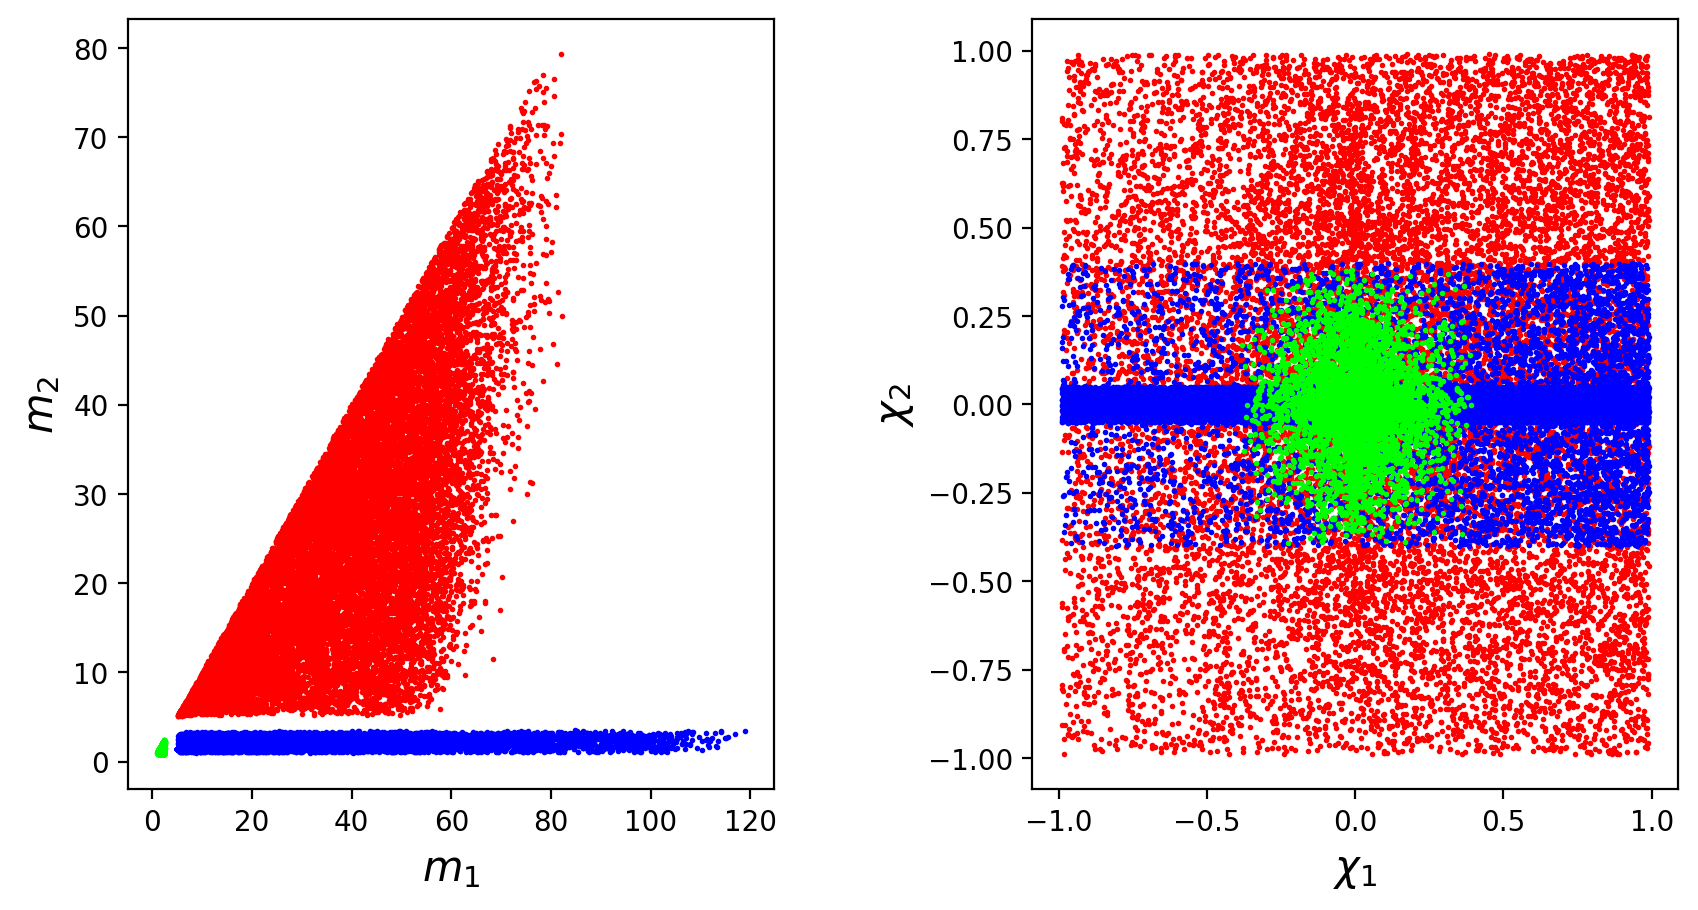
\includegraphics[width=0.45\textwidth]{training_parameter_space.png}
    \caption{The $m_1$-$m_2$ (left) and $\chi_1$-$\chi_2$ (right) parameter space 
		    of injections from the O2 MDC. \sa{changed colors according to BBH, BNS, BHNS
		    (maybe R-G-B is not the nicest choice possible)}
            }
	\label{parameter_space}
\end{figure}

\lorena{ML algorithms require the data to be standardized, i.e. have a zero
mean and unit variance. However, before standardizing the data we take an 
additional step to ensure astrophysical values from the predictions. In other 
words, a prediction without proper data conditioning can result in negative
masses and spin magnitudes greater than one. To avoid this, we first map the 
data to be in the $(0,1)$ range by solving a simple, linear system of equations 
separately for the masses and the spins. We, then, transform our data using a 
sigmoid function so that the values map between $(-\infty,+\infty)$. It
is only at this point that the data is ready to be standardized and fed into
GPR and NN. Once the algorithm gives us the predicted data, or the corrected
paramters estimates, the reverse process is applied, i.e., the data is scaled 
back from standardization, exponentiated, and mapped back to from $(0,1)$ to
physical values.}

%\footnote{We may want to add a footnote here and there.}

\section{Methods}
\label{sec:methods}

\lorena{For a given problem, there are different machine learning algorithms
that one can use to approximate a solution. For our purposes, we found 
Gaussian Process Regression and Neural Networks to be the most suitable methods
due to their interpretability and accuracy, respectively.}

\subsection{Gaussian Process Regression (GPR)}

\lorena{Gaussian process regression is a sophisticated mathematical tool to find joint
Gaussian distributions between system data and the predictions. This makes it a
particularly powerful in interpolating between data sets and estimating
errors. Throughout this paper, we use \texttt{PyTorch}'s GPR module. We have to
make certain choices for our model such as the kernel function, loss function,
and the number of iterations.}

\lorena{A kernel funciton is a covariance function use to measure the similarity
between two data points. Our choice of kernel for training is the radial 
basis function (RBF) which is a squared exponential function given by}
\begin{equation}
K(X_1, X_2) = e^{-\frac{||X_1-X_2||^2}{2 \sigma^2}},
\end{equation}
\lorena{where $X_1$ and $X_2$ are input data points and $\sigma$ is the variance, 
or lengthscale parameter. This kernel is chosen for its accuracy and speed. 
The predictions of the O2 dataset are not strongly depend on the choice of
kernel. Apart from its popularity due to its versatility, the RBF kernel seems
to perform slightly better than other kernels and without a large loss in
speed. The loss function we use is negative marginal log-likelihood and we
train for 20 iterations. The Adams optimizer is used to find the optimal 
hyperparameters with a learning rate of $0.1$. This combination of learning 
rate and iterations allows us to decrease the loss function at a quick rate 
without a decrease in accuracy.}

\subsection{Neural Networks (NNs)}
\simone{While deep NNs have been extensively used in recent years 
for classification tasks, in this work we consider a NN for our regression analysis.
We started by considering a NN implemented within the \texttt{TensorFlow} framework with 
\texttt{Keras} backend in order to have more flexibility in building the architecture of our NN. 
However we found that the best configurations between the ones tested is a standard
NN with two hidden layers with 400 neurons each, \texttt{ReLU} activation function, 
and a linear output function. Such configuration can be easily coded with \texttt{scikit-learn}
using the \texttt{MLPRegressor}. Since the \texttt{scikit-learn} is already imported 
in the LVK infrastructure, in the end we decide to use this framework.
We train our NN for 10 epochs using a batch size of 128, a learning rate of $10^{-3}$ and mean 
square error (MSE) loss function. 
}

\section{Results}

\begin{figure}
    \centering
    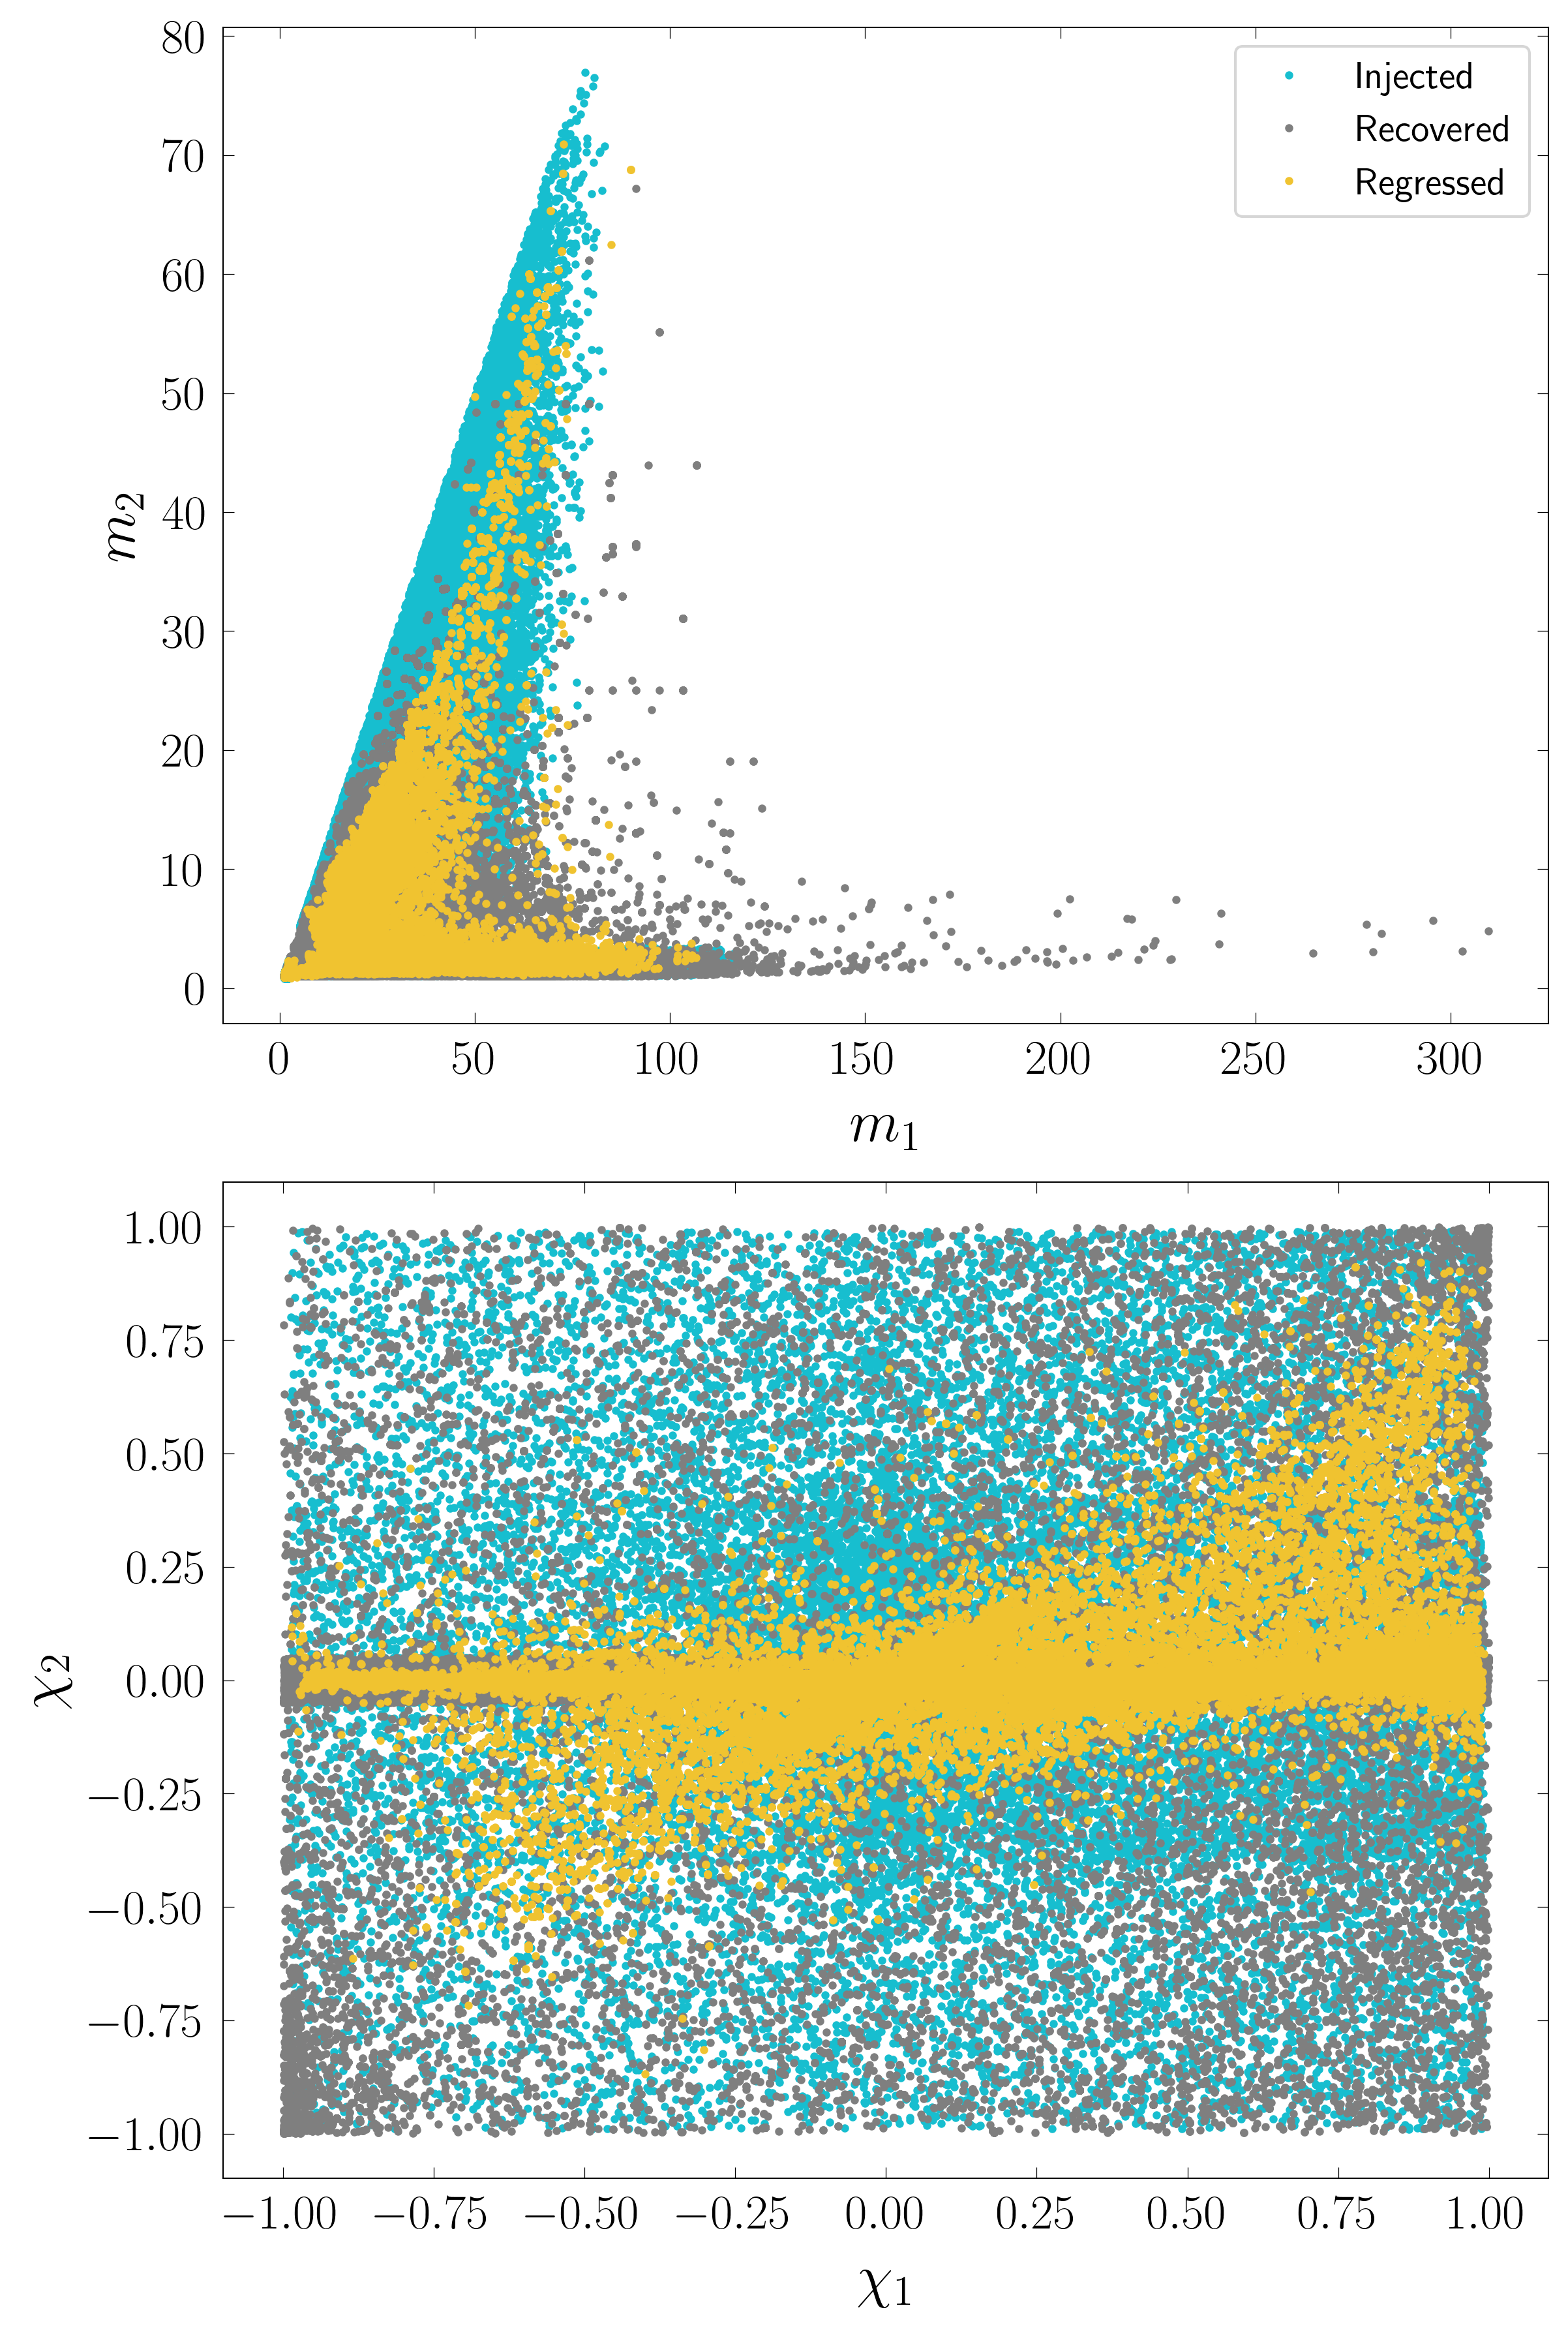
\includegraphics[width=0.45\textwidth]{inj_rec_pred_masses.png}
    \caption{The top panel shows the mass parameter space while the 
    		bottom panel shows the spin parameter space for the 
		injected (teal), recovered (gray), and regressed (yellow) 
		quantities. The regressed quantities shown here are using GPR.
            }
        \label{inj_rec_pred_masses}
\end{figure}

\begin{figure*}[t]
    \centering
    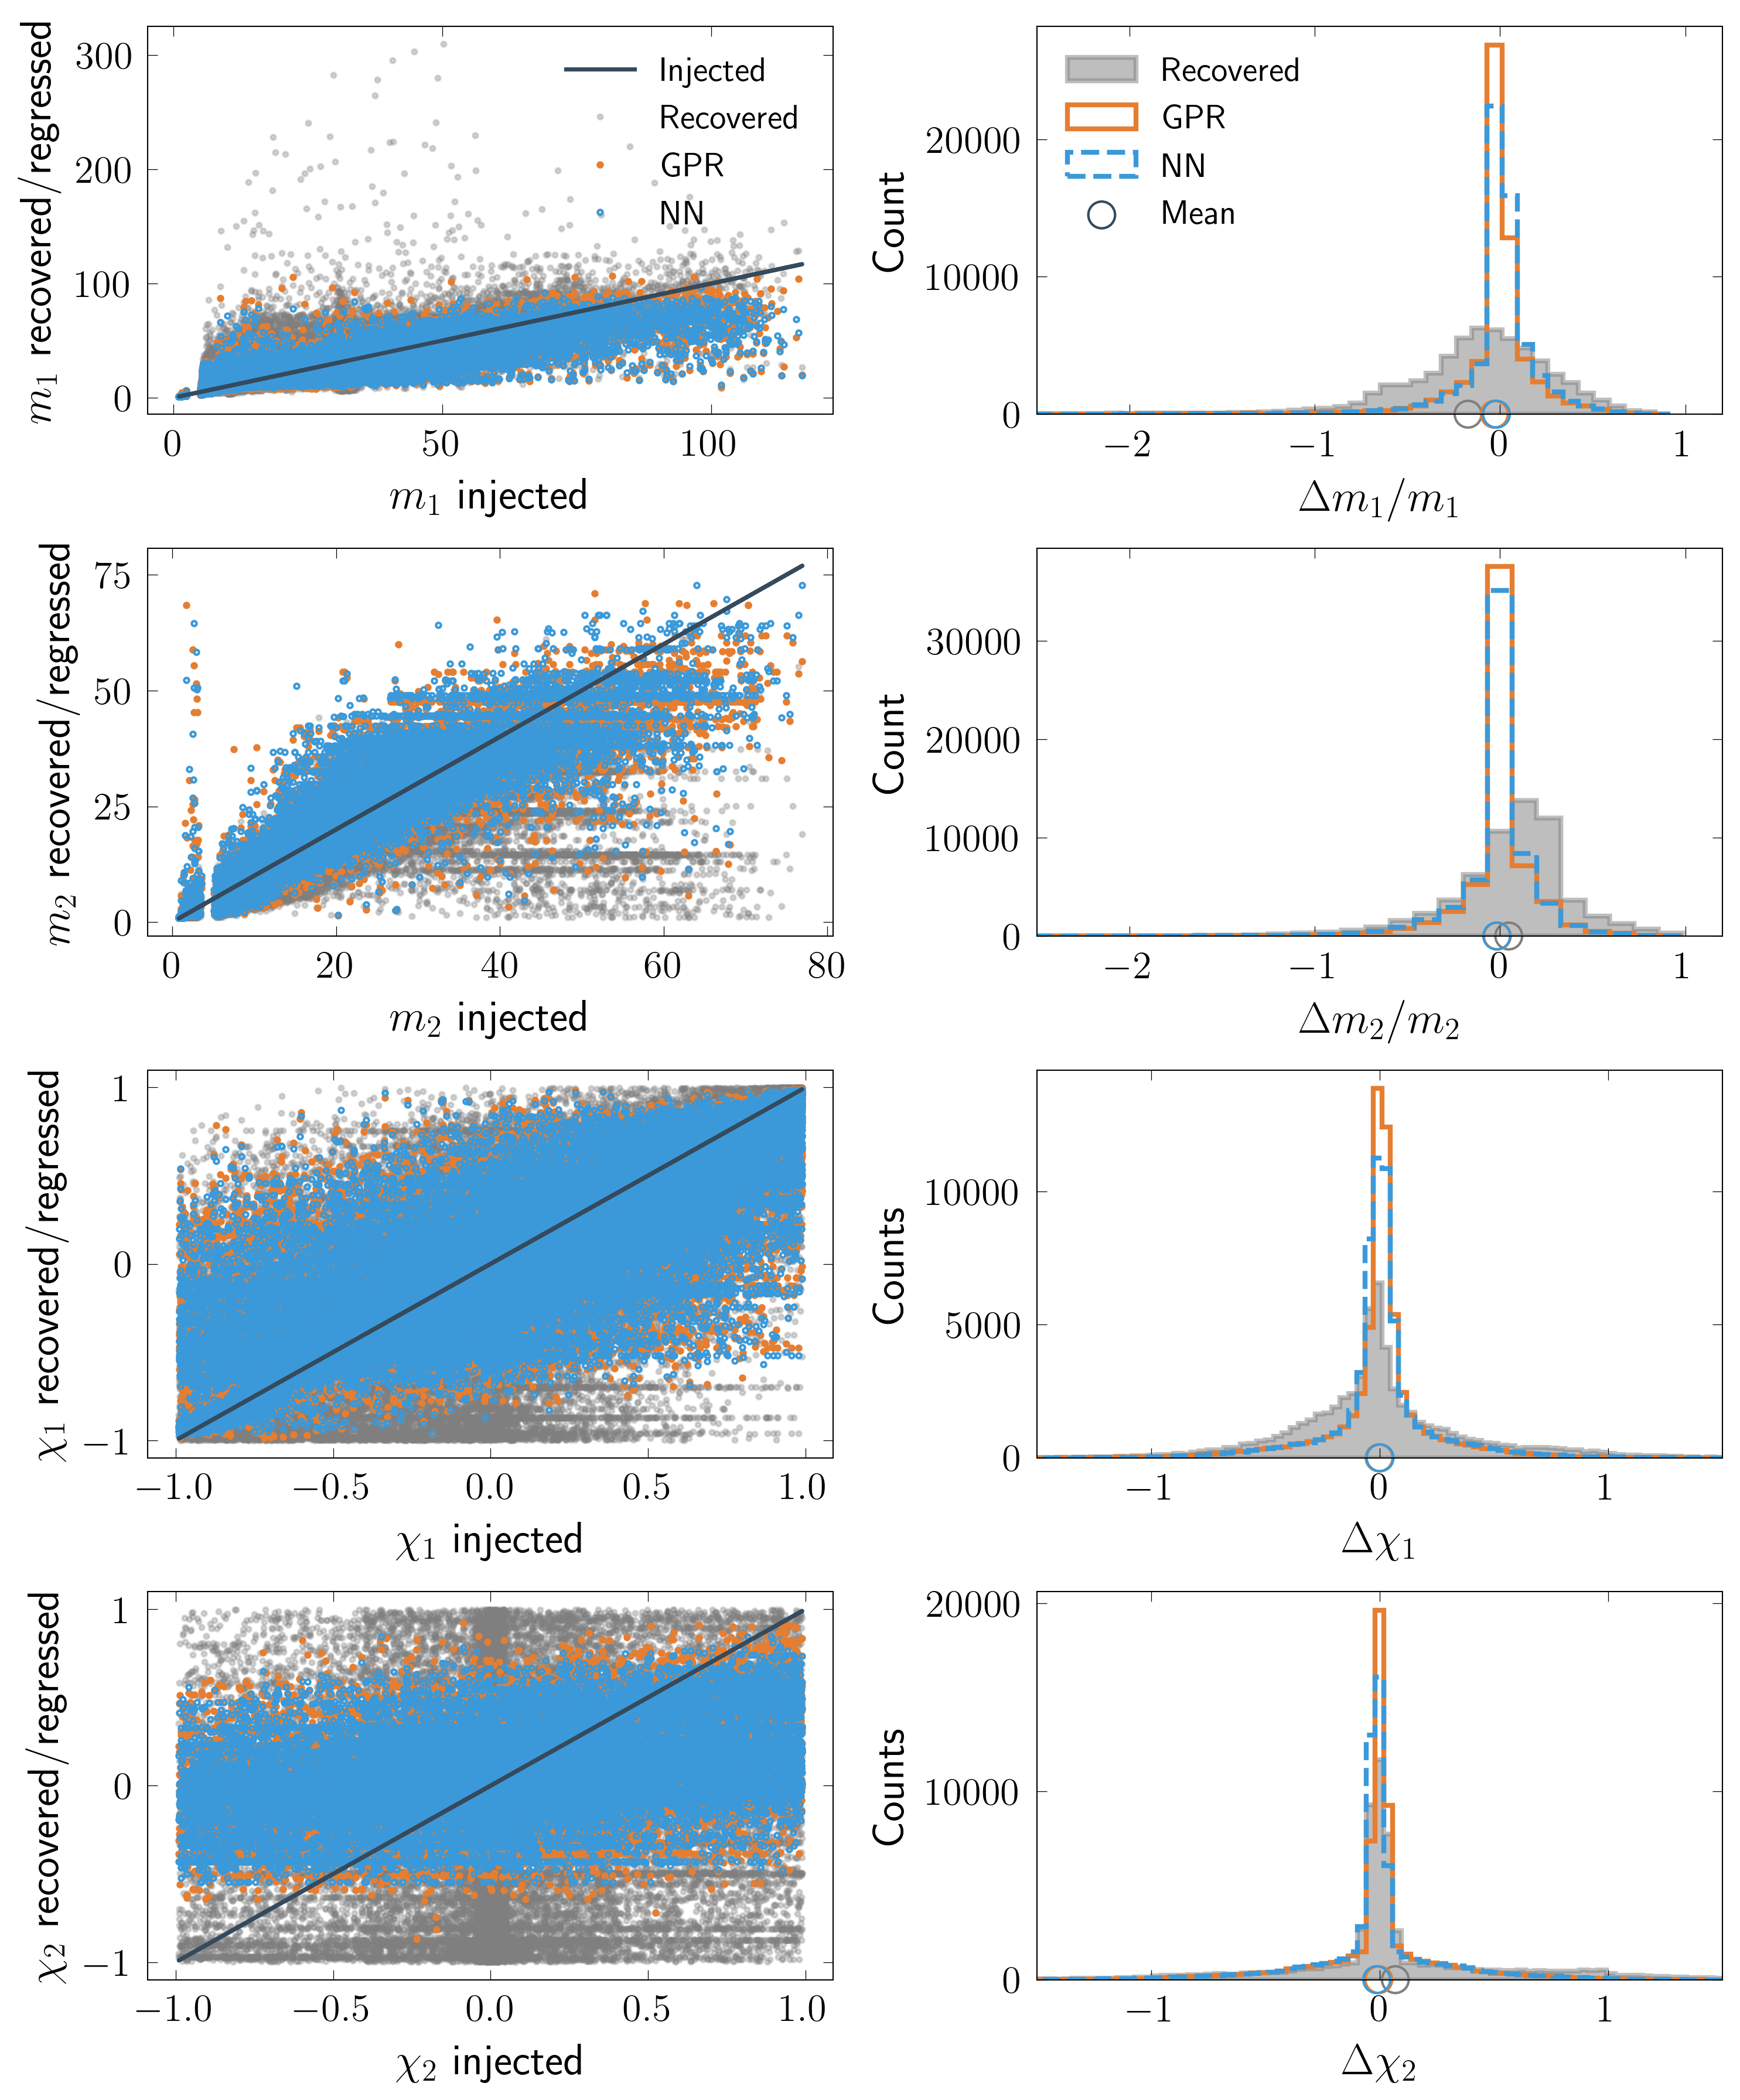
\includegraphics[width=\linewidth]{GPRvsNN_with_hist.png}
    \caption{The left side panels show the recovered (gray) and regressed
             masses and spins as functions of the injected values (solid line). 
             Regressed values from GPR are in orange while those from NN 
             are in blue. The right side panels show the mean error distributions.
            }
        \label{GPRvsNN}
\end{figure*}


\lorena{Using GPR and NNs to create a map between the injected and recovered
masses and spins of the O2 dataset allows us to better estimate the intrinsic 
parameters of a binary system. Fig.~\ref{inj_rec_pred_masses} shows the mass 
(top panel) and spin (bottom panel) parameter space of the injections along with 
the recovered parameters from \texttt{GstLAL} and the regressed values. 
Although regression does not fully cover the parameter space spanned by the 
injections, it mimics the features well. For example, compared to the injected 
binaries, the recovered mass values tend towards a high $m_1$ and low $m_2$, 
including several systems which are far from the expected mass-space. Instead, 
regression tries to correct for this tendency and includes the peak at high $m_2$ 
values without overestimating the $m_1$ range. The spin parameter-space is 
more complicated as most of the binaries include at least one 
non-spinning BH, and therefore, there is less training data for most of the spin 
parameter space. However, the regression algorithm notices this feature and so 
it mainly populates that area of spin-space.}

\lorena{We further break down regression results by directly comparing the 
closeness of the recovered/regressed quantities to the injected ones. In 
Fig.~\ref{GPRvsNN}, the gray circles represent the recovered values from the
best-fit template, the orange circles are the predictions coming from GPR, and
the blue circles are predictions from NN. The black lines shows where the
points would lie if the parameters where perfectly recovered and/or perfectly 
regressed. This figure shows how the primary mass is sometimes recovered as 
having very high values. With regression, however, one can correct for these more 
extreme cases and predict values that are closer to the injected values. Opposite 
to this overestimation, there is the underestimation of the secondary mass. 
Regardless of the values of the secondary mass injected, the recovered value 
tends to be more often underestimated. Regression is able to counteract this bias 
and decrease the difference with the injected values. Apart
from improving the mass estimates, one can see in the bottom left panels the effects
regression has on spins. Although both the recovered and regressed values
constitute wide bands around the injected values, the regressed values follow
the diagonal line closer. In the secondary spin, the areas of parameter space
furthest away from the true injected values are only populated by recovered
values but not regressed values.}

\lorena{To get a better understanding on the distribution of errors for these four
quantities, we show the mean relative error for the masses (top panels) and the
mean difference for the spins (bottom panels). It is evident that the error
distributions in all cases are more highly picked towards zero when using
regression. In addition, we show the mean of the error distributions on the 
horizontal axis. Table~\ref{tab:errors} quantify this errors. Greater
improvements are in the primary mass where errors drop from $35.2 \%$ to $12.7
\%$. The secondary mass still sees a decrease in mean percent error by about
$14.5 \%$. The mean absolute differences in the spins also decrease by about
half.}

%%\begin{table}
%%  \caption{\label{GPR_errors}  GPR. Mean differences in absolute value
%%    $|\Delta \bar{y}|=  \frac{1}{N} \Sigma |y^i_{\rm inj} - y^i_{\rm rec/pred}|$
%%    and averages of the relative differences in absolute value
%%    $|\delta \bar{y}| = \frac{1}{N} \Sigma \left( |y^i_{\rm inj} -
%%    y^i_{\rm rec/pred}|/y^i_{\rm inj} \right) $ for recovered and predicted data.
%%    For spin variables, the standard deviation $\sigma_y$ is computed from the
%%    former, while for mass variables is computed from the latter. Note that
%%    ${\cal{M}}_c$ is not predicted by the NN but it is computed from the
%%    predicted $m_i$.}
%%  \begin{center}
%%  \begin{tabular}{c|ccc|ccc}
%%  \hline\hline
%%  & $|\Delta \bar{y}_{\rm rec}|$  & $|\delta \bar{y}_{\rm rec}|$  & $\sigma_y^{\rm rec}$ &
%%     $|\Delta \bar{y}_{\rm pred}|$ & $|\delta \bar{y}_{\rm pred}|$ & $\sigma_y^{\rm pred}$ \\
%%  \hline\hline
%%$m_1$          & $6.625$ & $0.352$ & $0.511$ & $3.241$ & $0.127$ & $0.279$ \\
%%$m_2$          & $2.761$ & $0.256$ & $0.245$ & $1.414$ & $0.111$ & $0.319$ \\
%%$\chi_1$       & $0.266$ &  /  & $0.282$ & $0.134$ &  /  & $0.194$ \\
%%$\chi_2$       & $0.277$ &  /  & $0.373$ & $0.151$ &  /  & $0.225$ \\
%%\hline
%%${\cal{M}}_c$  & $1.323$ & $0.039$ & $0.099$ & $0.712$ & $0.027$ & $0.079$ \\
%%  \hline\hline
%%  \end{tabular}
%%  \end{center}
%%\end{table}
%%
%%\begin{table}
%%  \caption{\label{GPR_errors_temp} GPR. Same as Table~\ref{GPR_errors} but predicting $(m_1, {\cal{M}}_c, \chi_1, \chi_2)$. }
%%  \begin{center}
%%  \begin{tabular}{c|ccc|ccc}
%%  \hline\hline
%% %& $\bar{|\Delta y_{\rm rec}|}$ & $\bar{|\Delta y_{\rm rec}/y|}$ & $\bar{|\sigma_y_{\rm rec}|}$ & & &  \\
%%  & $|\Delta \bar{y}_{\rm rec}|$  & $|\delta \bar{y}_{\rm rec}|$  & $\sigma_y^{\rm rec}$ & 
%%     $|\Delta \bar{y}_{\rm pred}|$ & $|\delta \bar{y}_{\rm pred}|$ & $\sigma_y^{\rm pred}$ \\
%%  \hline\hline
%%$m_1$          & $6.625$ & $0.352$ & $0.511$ & $3.247$ & $0.127$ & $0.276$ \\
%%${\cal{M}}_c$  & $1.323$ & $0.039$ & $0.099$ & $0.704$ & $0.027$ & $0.086$ \\
%%$\chi_1$       & $0.266$ &  /  & $0.282$ & $0.135$ &  /  & $0.193$ \\
%%$\chi_2$       & $0.277$ &  /  & $0.373$ & $0.151$ &  /  & $0.225$ \\
%%\hline
%%$m_2$          & $2.761$ & $0.256$ & $0.245$ & $1.407$ & $0.114$ & $0.351$ \\
%%  \hline\hline
%%  \end{tabular}
%%  \end{center}
%%\end{table}

%%%%%% NN stuff pasted below %%%%%%%%

%\begin{figure}
%% >> python3 paper_plots.py --NN -v --plots rec_vs_pred
%    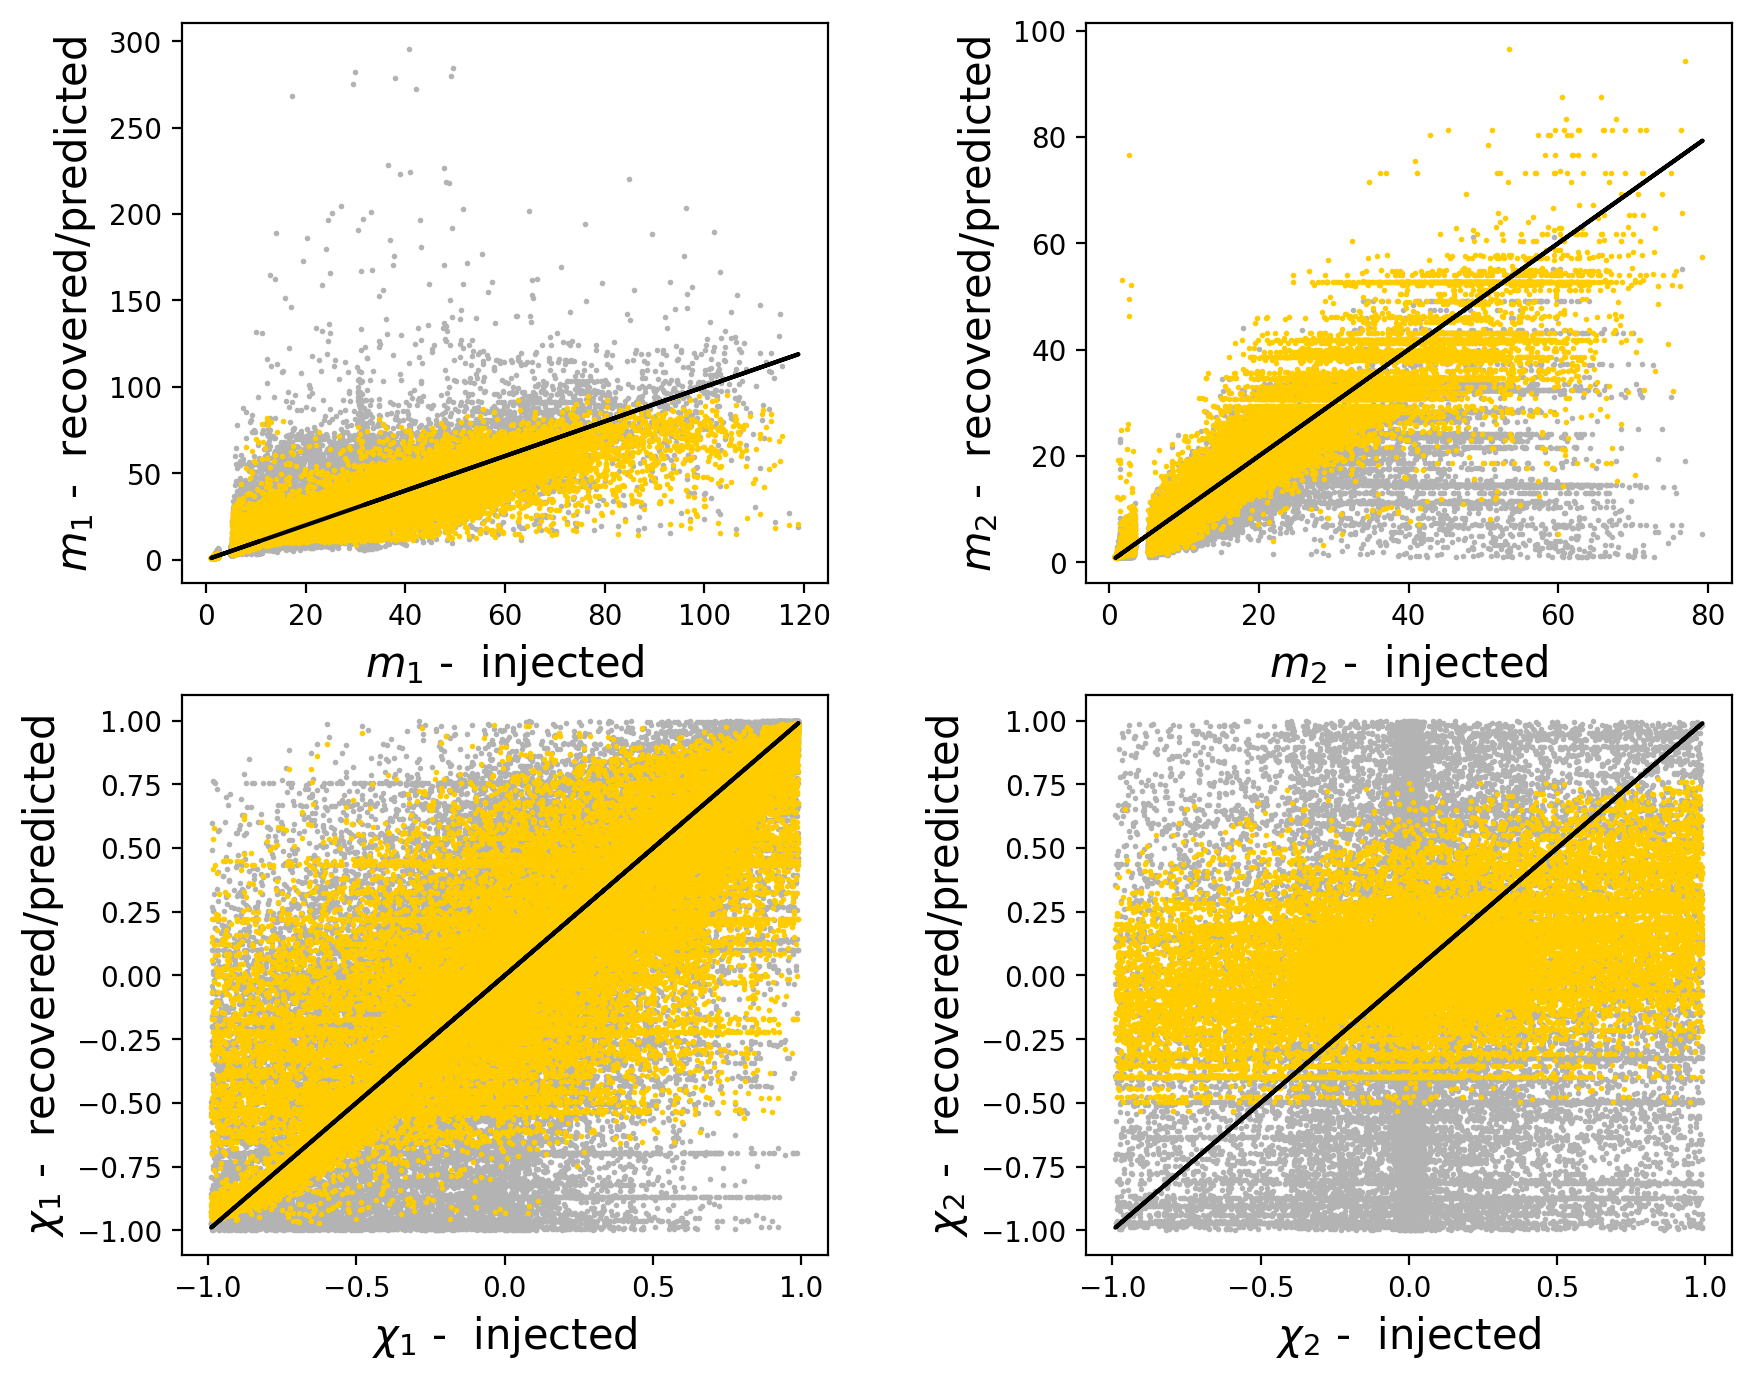
\includegraphics[width=0.45\textwidth]{m1m2chi1chi2_NN_recvspred.png}
%    \caption{NN version of Fig.~\ref{m_chi_comparisons}}
%        \label{m1m2chi1chi2_NN_recvspred}
%\end{figure}

%\begin{figure}
%% >> python3 paper_plots.py --NN -v --plots histo --histo_logs 1 1 0 0 --histo_fmin -10 -10 -2 -2
%    \centering
%    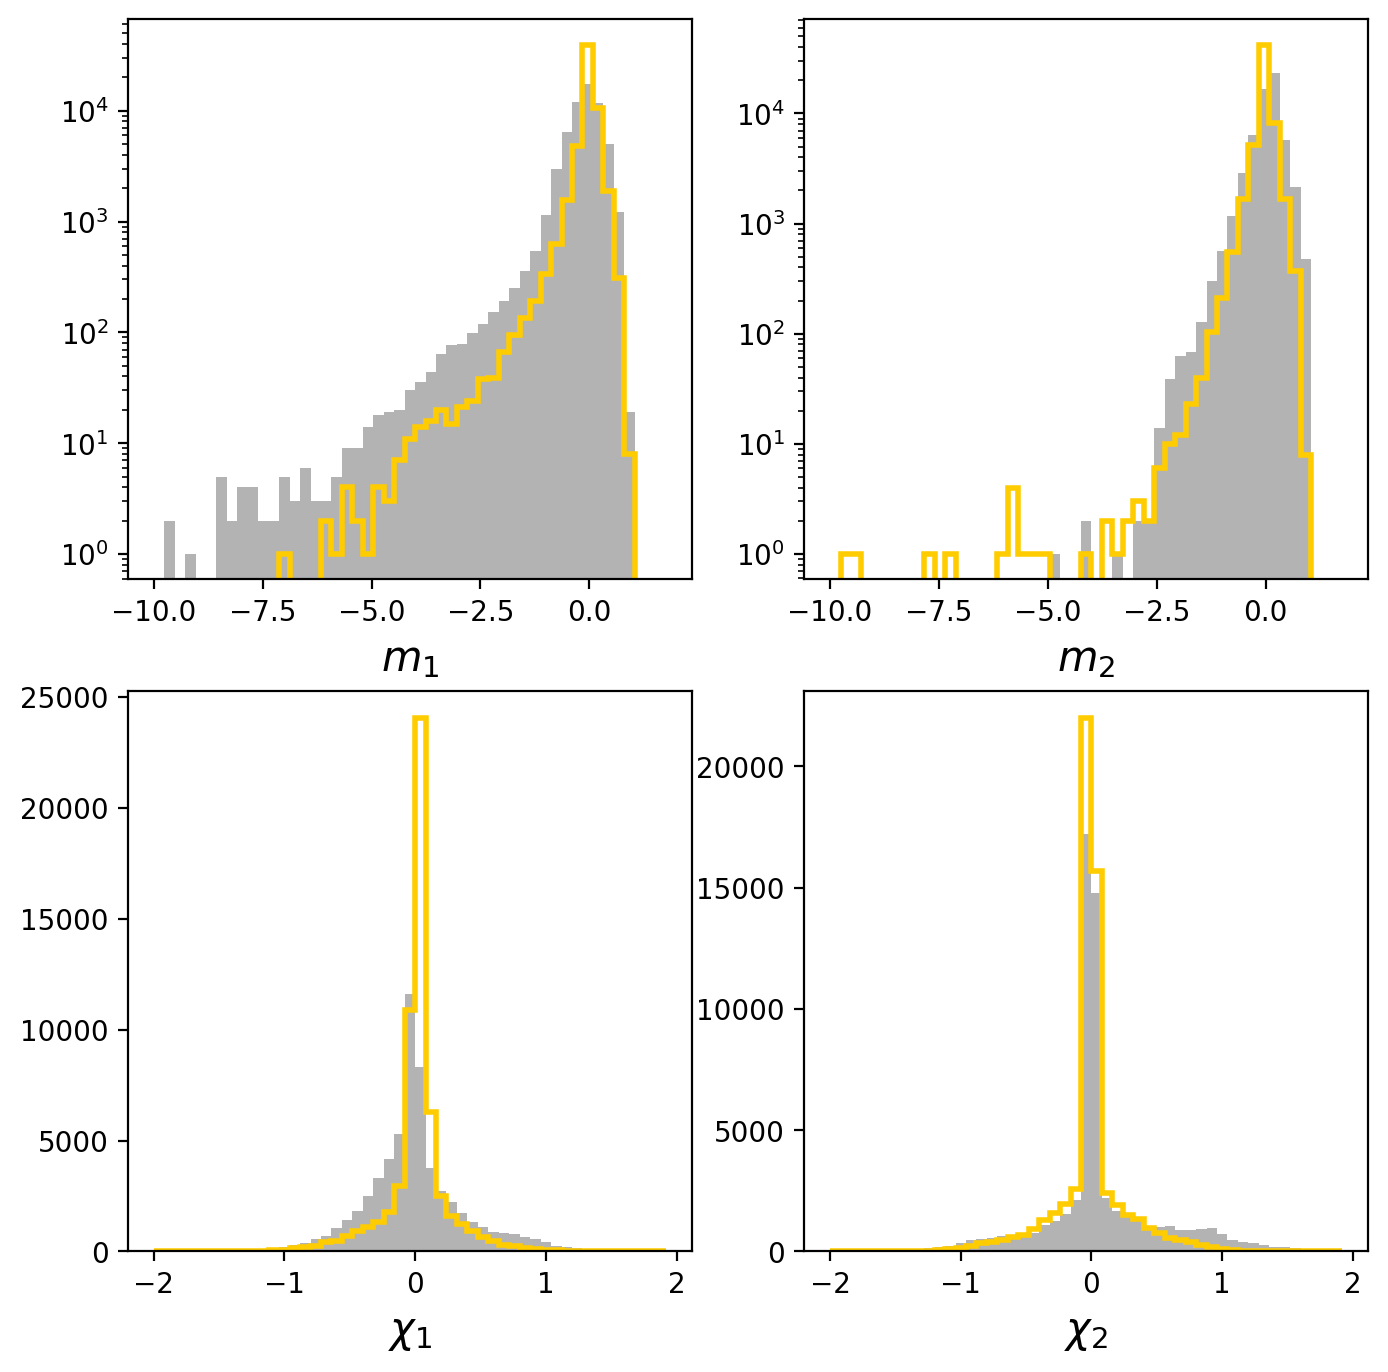
\includegraphics[width=0.45\textwidth]{m1m2chi1chi2_NN_histo.png}
%    \caption{Histograms}
%        \label{m1m2chi1chi2_NN_histo}
%\end{figure}

\begin{table*}
% >> python3 paper_plots.py --NN -v --errortab --tab_format tex --vars m1m2chi1chi2
  \caption{\label{tab:errors}  Mean differences in absolute value $|\Delta \bar{y}|=  \frac{1}{N} \Sigma |y^i_{\rm inj} - y^i_{\rm rec/pred}|$
  and averages of the relative
  differences in absolute value $|\delta \bar{y}| = \frac{1}{N} \Sigma \left( |y^i_{\rm inj} - y^i_{\rm rec/pred}|/y^i_{\rm inj} \right) $ for recovered and predicted data.
 The standard deviation  $\sigma^{\Delta y}$ and $\sigma^{\delta y}$ are computed, respectively, from the difference and relative difference distributions 
 without absolute value. Note that ${\cal{M}}_c$ is not directly predicted but it is computed from the predicted  masses $m_i$.}
  \begin{center}
  \begin{tabular}{c|cccc|cccc|cccc}
  \hline\hline
  & $|\Delta \bar{y}_{\rm rec}|$   & $\sigma_{\rm rec}^{\Delta y}$  & $|\delta \bar{y}_{\rm rec}|$  & $\sigma_{\rm rec}^{\delta y}$   &
      $|\Delta \bar{y}_{\rm nn}|$   & $\sigma_{\rm nn}^{\Delta y}$   & $|\delta \bar{y}_{\rm nn}|$   & $\sigma_{\rm nn}^{\delta y}$  &
      $|\Delta \bar{y}_{\rm gpr}|$  & $\sigma_{\rm gpr}^{\Delta y}$  & $|\delta \bar{y}_{\rm gpr}|$  & $\sigma_{\rm gpr}^{\delta y}$  \\
  \hline\hline
$m_1$          & $6.625$ & $12.052$ & $0.352$ & $0.596$ & $3.456$ & $6.976$ & $0.134$ & $0.292$ & 3.241 & ... & 0.127 & 0.279\\
$m_2$          & $2.761$ & $7.178$ & $0.256$ & $0.351$ & $1.457$ & $3.583$ & $0.123$ & $0.331$   &1.414  & ... & 0.111 & 0.319 \\
$\chi_1$       & $0.266$ & $0.388$ &  /  &  /  & $0.138$ & $0.236$ &  /  &  /  & 0.134 & 0.194 & / &  / \\
$\chi_2$       & $0.277$ & $0.460$ &  /  &  /  & $0.153$ & $0.268$ &  /  &  /  & 0.151 & 0.225 & / & / \\
\hline
${\cal{M}}_c$  & $1.323$ & $4.687$ & $0.039$ & $0.104$ & $0.769$ & $2.285$ & $0.036$ & $0.087$  & 0.712 & ... & 0.027 & 0.079\\
  \hline\hline
\end{tabular}
\end{center}
\end{table*}



\section{Confidence Intervals}
\label{sec:confintervals}

\simone{We compute confidence intervals in some way.}


\section{Conclusions}
%Information regarding future work and prelimiary results with O3:
%O3 MDC data contains $18,311$ systems which are recovered by the 
%\texttt{PyCBC}, \texttt{GstLAL}, and \texttt{MBTAOnline} pipelines. 
%The number of triggers recovered by these three detection pipelines 
%are $8,742$, $7,221$, and $2,348$, respectively.}

Reiterate why what we did is important and how it improves current knowledge.


\section*{Acknowledgments}
\lorena{We thank Deep Chatterjee and Shaon Ghosh for useful discussions and for
sharing their work, which helped us compare our results to those 
of~\cite{Chatterjee:2019avs}.}
%We also thank X, Y, and Z for reviewing an earlier version of this manuscript. 

\lorena{Part of this research was performed while the authors were visiting the Institute 
of Pure and Applied Mathematics (IPAM) at the University of California Los-Angeles 
(UCLA). The authors would like to thank IPAM, UCLA, and the National Science 
Foundation through grant DMS-1925919 for their warm hospitality during the fall of 
2021.}
%

\lorena{The authors are grateful for computational resources provided by the LIGO 
Laboratory and supported by the U.S. National Science Foundation Grants 
PHY-0757058 and PHY-0823459, as well as resources from the Gravitational Wave
Open Science Center, a service of the LIGO Laboratory, the LIGO Scientific 
Collaboration and the Virgo Collaboration. L.M.Z. would like to express
gratitude to the Mississippi Center for Supercomputing Research at the
University of Mississippi for support in computing resources.}
%

\lorena{The work of L.M.Z. was partially supported by the MSSGC Graduate
Research Fellowship, awarded through the NASA Cooperative Agreement
80NSSC20M0101.}
%The work of X.Y. was partially supported by NSF Grant No.~PHY-20XXXXX.
%

All plots were made using the python package \texttt{matplotlib}~\cite{Hunter:2007ouj}.

This manuscript has been assigned LIGO Document Control Center number LIGO-P22XXXXX.



\def\bibsection{\section*{References}}

\bibliography{regression}

\end{document}

% Local Variables:
% mode: latex
% End:
